\documentclass[../book.tex]{subfiles}
\begin{document}

    \subsection{函数的概念与特性}

    \subsubsection{函数$y = f(x)$}

    \begin{enumerate}
        \item \textbf{定义}：设 $D$ 是一个非空数集，如果存在一个对应法则 $f$，使得对于 $D$ 中的每一个数 $x$，都有唯一确定的数 $y$ 与之对应，则称 $f$ 为定义在 $D$ 上的\textbf{函数}，记作 $y = f(x)$。
        \begin{itemize}
            \item $D$ 称为函数的\textbf{定义域}
            \item $y$ 的全体称为函数的\textbf{值域}
            \item 函数的两个要素：\textbf{定义域}和\textbf{对应法则}
        \end{itemize}

        \item \textbf{函数的表示方法}：
        \begin{itemize}
            \item 解析法（公式法）
            \item 表格法
            \item 图像法
        \end{itemize}

        \item \textbf{分段函数}：在定义域的不同区间内用不同的表达式表示的函数。

        \item \textbf{常用函数类型}：
        \begin{itemize}
            \item 基本初等函数：幂函数、指数函数、对数函数、三角函数、反三角函数
            \item 初等函数：由基本初等函数经过有限次四则运算和复合运算得到的函数
        \end{itemize}
    \end{enumerate}

    \subsubsection{反函数$y = f^{-1}(x)$}

    \begin{enumerate}
        \item \textbf{定义}：设函数 $y = f(x)$ 的定义域为 $D$，值域为 $W$。若对于 $W$ 中的每一个 $y$ 值，在 $D$ 中都有唯一确定的 $x$ 值与之对应，则 $x$ 是 $y$ 的函数，称为 $y = f(x)$ 的\textbf{反函数}，记作 $x = f^{-1}(y)$ 或 $y = f^{-1}(x)$。

        \item \textbf{存在条件}：函数 $f(x)$ 存在反函数 $\Leftrightarrow$ $f(x)$ 是一一对应（单射）。

        \item \textbf{性质}：
        \begin{itemize}
            \item $f^{-1}[f(x)] = x$，$f[f^{-1}(x)] = x$
            \item 反函数的定义域是原函数的值域，反函数的值域是原函数的定义域
            \item $y = f(x)$ 与 $y = f^{-1}(x)$ 的图像关于直线 $y = x$ 对称
            \item 单调函数必有反函数，且反函数与原函数具有相同的单调性
        \end{itemize}

        \item \textbf{反函数的求法}：
        \begin{enumerate}
            \item 从 $y = f(x)$ 中解出 $x = f^{-1}(y)$
            \item 将 $x$ 换成 $y$，$y$ 换成 $x$，得到 $y = f^{-1}(x)$
        \end{enumerate}

        \item \textbf{经典反函数}：
        \begin{itemize}
            \item $\arcsin x$ 是 $\sin x$ 在 $[-\frac{\pi}{2}, \frac{\pi}{2}]$ 上的反函数
            \item $\arccos x$ 是 $\cos x$ 在 $[0, \pi]$ 上的反函数
            \item $\arctan x$ 是 $\tan x$ 在 $(-\frac{\pi}{2}, \frac{\pi}{2})$ 上的反函数
        \end{itemize}
    \end{enumerate}

    \subsubsection{复合函数$y = f[g(x)]$}

    \begin{enumerate}
        \item \textbf{定义}：设 $y = f(u)$ 的定义域为 $D_f$，$u = g(x)$ 的值域为 $W_g$，若 $D_f \cap W_g \neq \emptyset$，则 $y = f[g(x)]$ 称为由 $y = f(u)$ 和 $u = g(x)$ 复合而成的\textbf{复合函数}，$u$ 称为\textbf{中间变量}。

        \item \textbf{复合条件}：内层函数 $g(x)$ 的值域与外层函数 $f(u)$ 的定义域有交集。

        \item \textbf{复合函数的定义域}：使 $g(x)$ 的值落在 $f(u)$ 定义域内的所有 $x$ 的集合。

        \item \textbf{分解复合函数}：从外向内逐层分解，直到分解为基本初等函数。

        \item \textbf{例}：$y = \sin(2x + 1)$ 可分解为 $y = \sin u$，$u = 2x + 1$。
    \end{enumerate}

    \subsubsection{隐函数}

    \begin{enumerate}
        \item \textbf{定义}：如果变量 $x$ 和 $y$ 之间的函数关系是由方程 $F(x, y) = 0$ 所确定的，则称这种函数为\textbf{隐函数}。

        \item \textbf{显函数}：$y$ 能用 $x$ 的解析式直接表示，即 $y = f(x)$。

        \item \textbf{隐函数与显函数的关系}：
        \begin{itemize}
            \item 有些隐函数可以化为显函数（隐函数显化）
            \item 有些隐函数不能显化或显化困难
        \end{itemize}

        \item \textbf{隐函数求导}：对方程 $F(x, y) = 0$ 两边同时对 $x$ 求导，注意 $y$ 是 $x$ 的函数，需要使用链式法则。

        \item \textbf{例}：$x^2 + y^2 = 1$ 确定了 $y$ 是 $x$ 的隐函数。
    \end{enumerate}

    \subsubsection{四种特性}

    \paragraph{有界性}

    \begin{enumerate}
        \item \textbf{定义}：设函数 $f(x)$ 在数集 $D$ 上有定义。
        \begin{itemize}
            \item 若存在正数 $M$，使得对于所有 $x \in D$，都有 $|f(x)| \leq M$，则称 $f(x)$ 在 $D$ 上\textbf{有界}。
            \item 若存在常数 $M_1$，使得 $f(x) \geq M_1$（对所有 $x \in D$），则称 $f(x)$ 在 $D$ 上\textbf{有下界}。
            \item 若存在常数 $M_2$，使得 $f(x) \leq M_2$（对所有 $x \in D$），则称 $f(x)$ 在 $D$ 上\textbf{有上界}。
        \end{itemize}

        \item \textbf{重要结论}：$f(x)$ 在 $D$ 上有界 $\Leftrightarrow$ $f(x)$ 在 $D$ 上既有上界又有下界。

        \item \textbf{有界性的判断}：
        \begin{itemize}
            \item 利用定义直接判断
            \item 利用函数的性质（如 $\sin x$, $\cos x$ 在 $\mathbb{R}$ 上有界）
            \item 利用极限：$\lim\limits_{x \to x_0} f(x)$ 存在 $\Rightarrow$ $f(x)$ 在 $x_0$ 的某去心邻域内有界
            \item 闭区间上的连续函数必有界
        \end{itemize}

        \item \textbf{典型有界函数}：
        \begin{itemize}
            \item $|\sin x| \leq 1$，$|\cos x| \leq 1$
            \item $|\arctan x| < \frac{\pi}{2}$
            \item $\arcsin x \in [-\frac{\pi}{2}, \frac{\pi}{2}]$，$\arccos x \in [0, \pi]$
        \end{itemize}

        \item \textbf{注意}：有界性与区间有关，同一函数在不同区间上的有界性可能不同。
    \end{enumerate}

    \paragraph{单调性}

    \begin{enumerate}
        \item \textbf{定义}：设函数 $f(x)$ 在区间 $I$ 上有定义。
        \begin{itemize}
            \item 若对于 $I$ 中任意两点 $x_1 < x_2$，都有 $f(x_1) < f(x_2)$，则称 $f(x)$ 在 $I$ 上\textbf{单调递增}。
            \item 若对于 $I$ 中任意两点 $x_1 < x_2$，都有 $f(x_1) > f(x_2)$，则称 $f(x)$ 在 $I$ 上\textbf{单调递减}。
        \end{itemize}

        \item \textbf{判断方法}：
        \begin{itemize}
            \item \textbf{定义法}：取 $x_1 < x_2$，比较 $f(x_1)$ 与 $f(x_2)$
            \item \textbf{导数法}：$f'(x) > 0$ $\Rightarrow$ 单调递增；$f'(x) < 0$ $\Rightarrow$ 单调递减
        \end{itemize}

        \item \textbf{复合函数的单调性}：
        \begin{itemize}
            \item 增$\circ$增 $=$ 增
            \item 减$\circ$减 $=$ 增
            \item 增$\circ$减 $=$ 减
            \item 减$\circ$增 $=$ 减
            \item 口诀：\textbf{同增异减}
        \end{itemize}

        \item \textbf{单调性与反函数}：单调函数必有反函数，且反函数与原函数单调性相同。
    \end{enumerate}

    \paragraph{奇偶性}

    \begin{enumerate}
        \item \textbf{定义}：设函数 $f(x)$ 的定义域 $D$ 关于原点对称。
        \begin{itemize}
            \item 若对任意 $x \in D$，都有 $f(-x) = f(x)$，则称 $f(x)$ 为\textbf{偶函数}。
            \item 若对任意 $x \in D$，都有 $f(-x) = -f(x)$，则称 $f(x)$ 为\textbf{奇函数}。
        \end{itemize}

        \item \textbf{图像特征}：
        \begin{itemize}
            \item 偶函数图像关于 $y$ 轴对称
            \item 奇函数图像关于原点对称
        \end{itemize}

        \item \textbf{判断方法}：
        \begin{itemize}
            \item 定义法：计算 $f(-x)$ 与 $f(x)$ 的关系
            \item 图像法：观察对称性
        \end{itemize}

        \item \textbf{基本运算规律}：
        \begin{itemize}
            \item 偶 $+$ 偶 $=$ 偶，奇 $+$ 奇 $=$ 奇
            \item 偶 $-$ 偶 $=$ 偶，奇 $-$ 奇 $=$ 奇
            \item 偶 $\pm$ 奇 $=$ 不确定
            \item 偶 $\times$ 偶 $=$ 偶，奇 $\times$ 奇 $=$ 偶
            \item 偶 $\times$ 奇 $=$ 奇
        \end{itemize}

        \item \textbf{复合函数的奇偶性}：
        \begin{itemize}
            \item $f[\varphi(x)]$：内偶则偶，内奇同外
        \end{itemize}

        \item \textbf{与导数的关系}：
        \begin{itemize}
            \item 奇函数求导得偶函数
            \item 偶函数求导得奇函数
            \item 口诀：\textbf{求导一次，奇偶性互换}
        \end{itemize}

        \item \textbf{与积分的关系}：
        \begin{itemize}
            \item 若 $f(x)$ 为奇函数，则 $\int_0^x f(t)\,dt$ 为偶函数
            \item $\int_{-a}^{a} f(x)\,dx = \begin{cases}
                                                0, & f(x) \text{ 为奇函数} \\ 2\int_0^a f(x)\,dx, & f(x) \text{ 为偶函数}
            \end{cases}$
        \end{itemize}

        \item \textbf{重要性质}：
        \begin{itemize}
            \item 任意定义在关于原点对称区间上的函数，都可表示为一个奇函数与一个偶函数之和：
            \[
                f(x) = \underbrace{\frac{f(x) + f(-x)}{2}}_{\text{偶函数}} + \underbrace{\frac{f(x) - f(-x)}{2}}_{\text{奇函数}}
            \]
        \end{itemize}

        \item \textbf{常见奇函数}：
        \begin{itemize}
            \item $x$, $x^3$, $\sin x$, $\tan x$, $\arcsin x$, $\arctan x$
            \item $\ln\displaystyle\frac{1-x}{1+x}$, $\displaystyle\frac{1}{2^x + 1} - \frac{1}{2}$
            \item $\ln(x + \sqrt{x^2 + 1})$（反双曲正弦函数）
        \end{itemize}

        \item \textbf{常见偶函数}：
        \begin{itemize}
            \item $x^2$, $x^4$, $\cos x$, $|x|$
        \end{itemize}
    \end{enumerate}

    \paragraph{周期性}

    \begin{enumerate}
        \item \textbf{定义}：设函数 $f(x)$ 的定义域为 $D$。若存在非零常数 $T$，使得对于任意 $x \in D$，有 $x + T \in D$ 且
        \[
            f(x + T) = f(x),
        \]
        则称 $f(x)$ 为\textbf{周期函数}，$T$ 称为 $f(x)$ 的\textbf{周期}。

        \item \textbf{最小正周期}：若周期函数的所有正周期中存在最小值，则称此最小值为\textbf{最小正周期}。

        \item \textbf{常见周期函数及其周期}：
        \begin{itemize}
            \item $\sin x$, $\cos x$：周期 $2\pi$
            \item $\tan x$, $\cot x$：周期 $\pi$
            \item $|\sin x|$, $|\cos x|$：周期 $\pi$
            \item $\sin\omega x$, $\cos\omega x$：周期 $\displaystyle\frac{2\pi}{|\omega|}$
        \end{itemize}

        \item \textbf{周期的性质}：
        \begin{itemize}
            \item 若 $T$ 是 $f(x)$ 的周期，则 $kT$（$k \in \mathbb{Z}, k \neq 0$）也是 $f(x)$ 的周期
            \item 若 $f(x)$ 以 $T$ 为周期，则 $f(ax + b)$ 以 $\displaystyle\frac{T}{|a|}$ 为周期
            \item 若 $f(x)$ 和 $g(x)$ 都以 $T$ 为周期，则 $f(x) \pm g(x)$, $f(x) \cdot g(x)$ 也以 $T$ 为周期（在定义域内）
        \end{itemize}

        \item \textbf{周期函数的积分}：
        \[
            \int_a^{a+T} f(x)\,dx = \int_0^T f(x)\,dx
        \]
        即周期函数在任意一个周期长度区间上的积分值相等。

        \item \textbf{特殊周期函数}：
        \begin{itemize}
            \item $f(x) = x - [x]$（取整函数的小数部分）：周期 $1$
            \item 狄利克雷函数 $D(x) = \begin{cases}
                                           1, & x \in \mathbb{Q} \\ 0, & x \notin \mathbb{Q}
            \end{cases}$：任意非零有理数都是其周期（无最小正周期）
        \end{itemize}
    \end{enumerate}

    \subsubsection{基础概念}

    \begin{enumerate}
        \item 反双曲正弦函数: $y = \ln\left(x + \sqrt{x^2 + 1}\right)$，常见的奇函数
        \begin{itemize}
            \item
            \[
                \frac{d}{dx}\,\ln\left(x + \sqrt{x^2 + 1}\right)
                = \frac{1}{\sqrt{1+x^2}}
            \]

            \item
            \[
                \int \frac{1}{\sqrt{1+x^2}}\,dx
                = \ln\left(x + \sqrt{x^2 + 1}\right) + C
            \]

            \item
            \[
                \int_{-1}^{1}
                \left[\ln\left(x + \sqrt{x^2 + 1}\right) + x^2\right]\,dx
                = \int_{-1}^{1} x^2\,dx
                = \frac{2}{3},
            \]
        \end{itemize}
        \item 双曲正弦函数: $\displaystyle y = \frac{e^x - e^{-x}}{2}$ \\
        \item 双曲余弦函数: $\displaystyle y = \frac{e^x + e^{-x}}{2}$ \\
        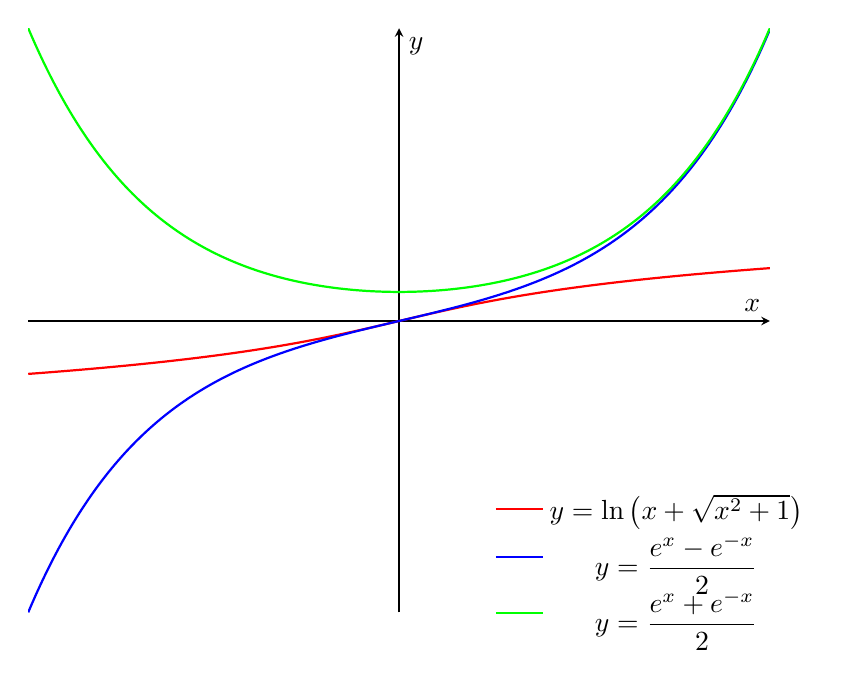
\begin{tikzpicture}
            \begin{axis}
                [
                xshift = -1.8cm,
                axis lines = middle,
                xlabel = {$x$},
                ylabel = {$y$},
                domain = -3:3,
                samples = 200,
                width = 11cm,
                height = 9cm,
                xtick = \empty,
                ytick = \empty,
                legend style={
                    at={(0.02,0.98)},
                    anchor=north west,
                    xshift=160pt,
                    yshift=-160pt,
                    draw=none
                }
                ]

                \addplot[red, thick] {ln(x + sqrt(x^2 + 1))};
                \addlegendentry{$y=\ln\left(x + \sqrt{x^2 + 1}\right)$}

                \addplot[blue, thick] {sinh(x)};
                \addlegendentry{$\displaystyle y=\frac{e^x - e^{-x}}{2}$}

                \addplot[green, thick] {cosh(x)};
                \addlegendentry{$\displaystyle y=\frac{e^x + e^{-x}}{2}$}

            \end{axis}
        \end{tikzpicture}
        \item 函数奇偶性
        \begin{itemize}
            \item $f(x) + f(-x)$必是偶函数
            \item $f(x) - f(-x)$必是奇函数
            \item 基本代数规则
            \begin{circlenum}
                \item 偶 + 偶 = 偶
                \item 奇 + 奇 = 奇
                \item 偶 + 奇 = 不知道
                \item 偶 $\cdot$ 偶 = 偶
                \item 奇 $\cdot$ 奇 = 偶
                \item 偶 $\cdot$ 奇 = 奇
            \end{circlenum}
            \item 任意定义在关于原点对称区间上的函数，都可以表示为一个奇函数与一个偶函数之和。对任一函数 $f(x)$，定义
            \[
                u(x) = \frac{1}{2}\bigl[f(x) + f(-x)\bigr], \qquad
                v(x) = \frac{1}{2}\bigl[f(x) - f(-x)\bigr].
            \]
            则有 $u(x)$ 是偶函数，$v(x)$ 是奇函数。并且
            \[
                f(x)
                = \frac{1}{2}\bigl[f(x) + f(-x)\bigr]
                + \frac{1}{2}\bigl[f(x) - f(-x)\bigr]
                = u(x) + v(x).
            \]
            \item $f[\varphi(x)]$内偶则偶，内奇同外
            \item $\color{red}{\bigstar}$求导一次，奇偶性互换
            \item $f(x)$奇$\Rightarrow \int_0^x f(t)\,\mathrm{d}t$偶
            \item 设对任意的$x, y$，都有$f(x + y) = f(x) + f(y)$，则$f(x)$是奇函数
            \item 常见的奇函数
            \begin{enumerate}
                \item $f(x) = \ln\displaystyle\frac{1-x}{1+x} = \ln(1-x) - \ln(1+x)$
                \item $f(x) = \displaystyle\frac{1}{2^x + 1} - \frac{1}{2}$
            \end{enumerate}
        \end{itemize}
        \item 反正弦函数 $y=\arcsin x$ 是函数
        \[
            y=\sin x \quad \left(x\in\left[-\frac{\pi}{2},\,\frac{\pi}{2}\right]\right)
        \]
        的反函数，其主值区间为
        \[
            \arcsin x \in \left[-\frac{\pi}{2},\,\frac{\pi}{2}\right].
        \]
        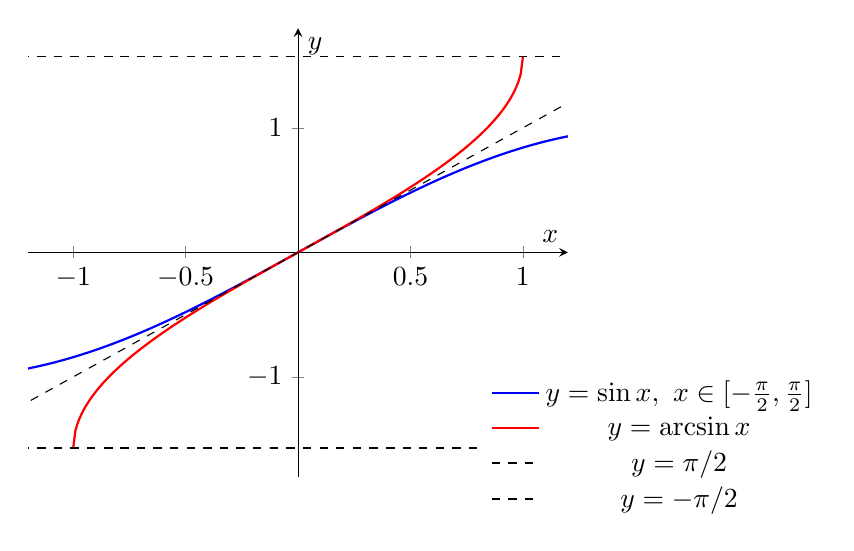
\begin{tikzpicture}
            \begin{axis}
                [
                axis lines = middle,
                xlabel = {$x$},
                ylabel = {$y$},
                xmin = -1.2, xmax = 1.2,
                ymin = -1.8, ymax = 1.8,
                samples = 200,
                legend style={
                    draw=none, at={(0.02,0.98)}, anchor=north west,
                    xshift=160pt,
                    yshift=-120pt,
                }]

% y = sin x (restricted)
                \addplot[blue, thick, domain=-pi/2:pi/2]
                {sin(deg(x))};
                \addlegendentry{$y=\sin x,\ x\in[-\frac{\pi}{2},\frac{\pi}{2}]$}

% y = arcsin x  ← 关键修正
                \addplot[red, thick, domain=-1:1]
                {asin(x)*pi/180};
                \addlegendentry{$y=\arcsin x$}

% y = x
                \addplot[dashed] {x};

                % y = \pi/2
                \addplot[dashed] {1.570796};
                \addlegendentry{$y=\pi/2$}

                % y = -\pi/2
                \addplot[dashed] {-1.570796};
                \addlegendentry{$y=-\pi/2$}
            \end{axis}
        \end{tikzpicture}

        若 $y = \sin x,\ x \in \left(\displaystyle \frac{\pi}{2}, \frac{3\pi}{2}\right)$，则$x = \pi - \arcsin y$
        \item 反余弦函数 $y=\arccos x$ 是函数
        \[
            y=\cos x \quad (x\in[0,\pi])
        \]
        的反函数，其主值区间为
        \[
            \arccos x \in [0,\pi].
        \]
        \begin{tikzpicture}
            \begin{axis}
                [
                axis lines = middle,
                xlabel = {$x$},
                ylabel = {$y$},
                xmin = -1.2, xmax = 1.2,
                ymin = -0.2, ymax = 3.4,
                samples = 200,
                legend style={draw=none, at={(0.02,0.98)}, anchor=north west,xshift=160pt}
                ]

% y = arccos x  ← 关键修正
                \addplot[red, thick, domain=-1:1]
                {acos(x)*pi/180};
                \addlegendentry{$y=\arccos x$}

            \end{axis}
        \end{tikzpicture}

    \end{enumerate}

    \subsubsection{结论}

    \begin{enumerate}
        \item 当$x \to 0$时，常用的等价无穷小
        \begin{itemize}
            \item $x \sim y = \ln\left(x + \sqrt{x^2 + 1}\right)$
            \item $x \sim \sin x$
            \item $x \sim \tan x$
        \end{itemize}
        \item $x-[x]$是$x$的小数部分，是以1为周期的函数
        \item 充分条件 \& 必要条件
        \begin{itemize}
            \item $Y$ 的必要条件 $\Rightarrow Y \Rightarrow$
            \item $X$ 是 $Y$ 的必要条件 $\Rightarrow Y \Rightarrow X$
            \item $Y$ 的充分条件 $\Rightarrow X \Rightarrow Y$
            \item $X$ 是 $Y$ 的充分条件 $\Rightarrow X \Rightarrow Y$
        \end{itemize}
    \end{enumerate}

    \subsubsection{定理}

    \begin{enumerate}
    \end{enumerate}

    \subsubsection{运算}

    \begin{enumerate}

    \end{enumerate}

    \subsubsection{公式}

    \begin{enumerate}
        \item $\displaystyle x^2 + \frac{1}{x^2} = (x + \frac{1}{x})^2 - 2$
        \item
        \[
            e^x = \sum_{n=0}^{\infty} \frac{x^n}{n!}.
        \]

        广义化：
        \[
            2^x = e^{x\ln 2}
            = \sum_{n=0}^{\infty} \frac{(x\ln 2)^n}{n!}.
        \]
        \item $[x + n] = [x] + n$.
        特别地，当 $n=1$ 时，$[x + 1] = [x] + 1$
    \end{enumerate}

    \subsubsection{方法总结}

    \begin{enumerate}

    \end{enumerate}

    \subsubsection{条件转换思路}

    \begin{enumerate}

    \end{enumerate}

    \subsubsection{理解}

    \begin{enumerate}
    \end{enumerate}
\end{document}
